\documentclass[10pt,a4paper]{article}
\usepackage[margin=2.2cm]{geometry}
\usepackage{amsmath,amssymb}
\usepackage{graphicx}
\usepackage{booktabs}
\usepackage{xcolor}
\usepackage{tikz}
\usetikzlibrary{arrows.meta,positioning,shapes.geometric,calc,fit,backgrounds}
\usepackage[font=small,labelfont=bf]{caption}
\usepackage{subcaption}
\usepackage{microtype}
\usepackage[section]{placeins}
\usepackage{enumitem}
\usepackage[hidelinks]{hyperref}

\definecolor{tmblue}{HTML}{2A78D6}
\definecolor{frorange}{HTML}{EB6834}
\definecolor{fraqua}{HTML}{1BAF7A}
\definecolor{ink2}{HTML}{52514E}
\definecolor{boxfill}{HTML}{EEF4FC}
\definecolor{warnfill}{HTML}{FDF0EA}

\setlist{itemsep=2pt,topsep=3pt}
\graphicspath{{figures/}}

\title{\textbf{TraceMaker}\\[2pt]\large A learning, GPU-assisted PCB autorouter and placer for KiCad\\[2pt]
\normalsize Design, method and benchmark results}
\author{Development report}
\date{2 October 2026}

\begin{document}
\maketitle

\begin{abstract}
\noindent TraceMaker reads KiCad 4--10 boards directly, routes them with an exact-geometry lattice router
that learns from its own failures, and writes the tracks and vias back into the \texttt{.kicad\_pcb} file
without disturbing anything else. It also places components with an analytic placer checked by the router.
Every result is judged by KiCad's own design-rule checker (\texttt{kicad-cli pcb drc}). On Freerouting's PCBench
benchmark set TraceMaker routes 100\% of the sampled tier-A boards cleanly, 65.0\% of tier B, 60.0\% of tier C and
54.5\% of tier D. Freerouting 2.5.0-RC12's published results on the same boards are 100\%, 50.0\%, 46.7\% and
36.4\%. No board in the final runs has a DRC error introduced by the router. On 60 boards never used during
development, with Freerouting 2.5.0-RC12 and 1.9.0 run on the same machine and judged by the same KiCad DRC,
TraceMaker's results are clean on 73--78\% of boards against 3\% and 32\%, with 5\% shorter tracks and 28\% fewer
bends than Freerouting 2.5, but more vias.
\end{abstract}

% ------------------------------------------------------------------------------------------------------------
\section{What TraceMaker does}

A printed circuit board (PCB) starts as a set of footprints with copper pads and a netlist that says which pads
must be connected. The router must draw copper tracks (and vias between layers) that make every connection while
respecting the board's design rules: minimum clearances between different nets, track widths, hole sizes, the
board edge, solder-mask openings and more. A route is only useful if the board then passes the design-rule check
(DRC) of the EDA tool the designer uses. TraceMaker therefore treats KiCad's DRC as the judge.

Figure~\ref{fig:beforeafter} shows the task on a real board from the benchmark set: a three-channel motor driver
with fine-pitch QFN packages. The left panel shows the input, with the required connections drawn as straight
airwires. The right panel shows TraceMaker's result, which KiCad's DRC reports as complete with no violations.

\begin{figure}[h]
  \centering
  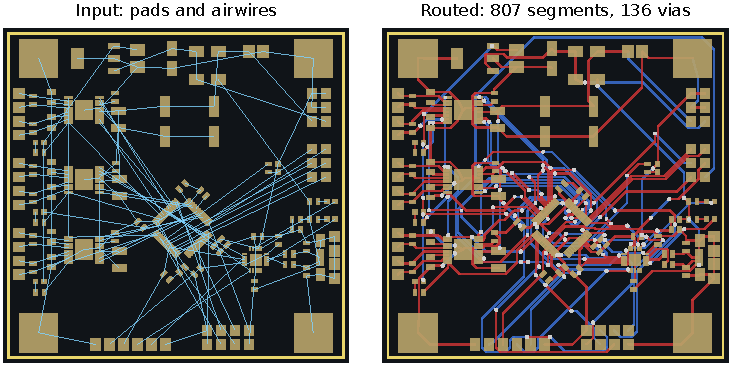
\includegraphics[width=\textwidth]{before_after.pdf}
  \caption{PCBench board \texttt{motor-3xdrv8833} (tier B, 195 connections). Left: input pads and airwires
  (a minimum spanning tree per net). Right: TraceMaker's routing on the front (red) and back (blue) copper,
  with vias in grey. KiCad's DRC: fully connected, no router-introduced violations.}
  \label{fig:beforeafter}
\end{figure}

% ------------------------------------------------------------------------------------------------------------
\section{Architecture}

TraceMaker is about 12,500 lines of C++20 and CUDA, plus a 2,000-line TypeScript viewer and Python tooling. It
runs on Ubuntu with an NVIDIA P100 and V100, but every GPU path has a CPU reference that gives identical results.
Figure~\ref{fig:arch} shows the pipeline.

\begin{figure}[h]
\centering
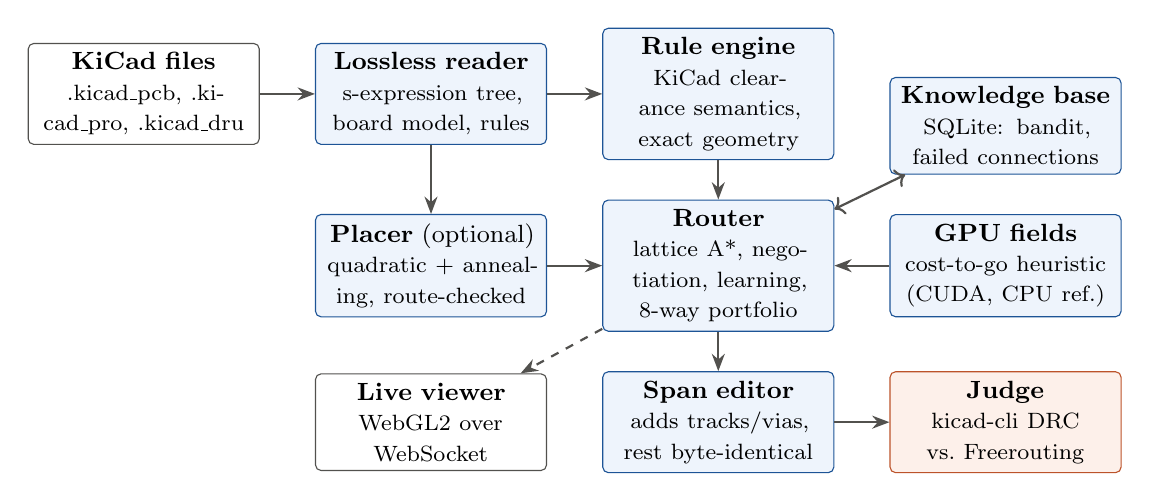
\begin{tikzpicture}[
  node distance=5mm and 7mm,
  blk/.style={draw=tmblue!70!black, fill=boxfill, rounded corners=2pt, align=center, font=\small,
              minimum height=10mm, text width=27mm},
  io/.style={blk, fill=white, draw=ink2},
  judge/.style={blk, fill=warnfill, draw=frorange!80!black},
  arr/.style={-{Stealth[length=2.2mm]}, thick, ink2}]
  \node[io] (in) {\textbf{KiCad files}\\ \footnotesize .kicad\_pcb, .kicad\_pro, .kicad\_dru};
  \node[blk, right=of in] (io) {\textbf{Lossless reader}\\ \footnotesize s-expression tree, board model, rules};
  \node[blk, right=of io] (drc) {\textbf{Rule engine}\\ \footnotesize KiCad clearance semantics, exact geometry};
  \node[blk, below=of drc] (route) {\textbf{Router}\\ \footnotesize lattice A*, negotiation, learning, 8-way portfolio};
  \node[blk, left=of route] (place) {\textbf{Placer} (optional)\\ \footnotesize quadratic + annealing, route-checked};
  \node[blk, right=of route] (gpu) {\textbf{GPU fields}\\ \footnotesize cost-to-go heuristic (CUDA, CPU ref.)};
  \node[blk, below=of route] (edit) {\textbf{Span editor}\\ \footnotesize adds tracks/vias, rest byte-identical};
  \node[io, left=of edit] (view) {\textbf{Live viewer}\\ \footnotesize WebGL2 over WebSocket};
  \node[judge, right=of edit] (judge) {\textbf{Judge}\\ \footnotesize kicad-cli DRC vs.\ Freerouting};
  \node[blk, above=of gpu] (kb) {\textbf{Knowledge base}\\ \footnotesize SQLite: bandit, failed connections};
  \draw[arr] (in) -- (io);
  \draw[arr] (io) -- (drc);
  \draw[arr] (drc) -- (route);
  \draw[arr] (place) -- (route);
  \draw[arr] (gpu) -- (route);
  \draw[arr, <->] (kb) -- (route);
  \draw[arr] (route) -- (edit);
  \draw[arr, dashed] (route) -- (view);
  \draw[arr] (edit) -- (judge);
  \draw[arr] (io) -- (place);
\end{tikzpicture}
\caption{TraceMaker pipeline. The router never commits copper that the exact rule engine has not verified; the
finished board is judged by KiCad's own DRC.}
\label{fig:arch}
\end{figure}

\paragraph{Lossless KiCad I/O.} The reader parses the board into an s-expression tree that remembers the byte span
of every node. Edits (adding a track, moving a footprint) replace or append spans; everything else is written back
byte for byte. All 3,538 fixture boards in the test set round-trip identically. The reader handles KiCad 4 to 10
formats, including legacy arcs, numbered and named nets, custom layer names and project rule files.

\paragraph{Exact geometry.} All coordinates are 64-bit integer nanometres, as in KiCad. Shapes are ``rounded
cores'': a point, segment or polygon inflated by a radius, which represents round pads, tracks, vias and rounded
rectangles exactly. Distance predicates use 128-bit integer arithmetic, so a clearance test never depends on
floating-point rounding.

\paragraph{A KiCad-equivalent rule engine.} Clearance is not a single number in KiCad. It is the maximum of the
board minimum, the net-class clearances of both items, local pad and footprint overrides, diff-pair gaps and
custom rules, with special cases for holes, the board edge and solder-mask openings. Each rule TraceMaker
implements was checked against \texttt{kicad-cli} on real boards (Section~\ref{sec:testing}). Examples found this
way include: plated through-holes are on every copper layer whatever the file says; non-plated holes carry the
board-edge clearance; a solder-mask opening exposes copper of its pad's net on both sides; mask graphics grow by
the board's mask expansion; copper text is an obstacle.

% ------------------------------------------------------------------------------------------------------------
\section{How the router works}

\subsection{Search on an octilinear lattice}

The board is covered by a lattice of points per copper layer. The pitch is a sixth of the smallest
\emph{track width + clearance} on the board (25--100\,\textmu m), so lattice tracks fit between fine-pitch pads.
From each point a track may move in eight directions (0\textdegree, 45\textdegree, 90\textdegree, \ldots) or
change layer through a via. A connection is found with A* search, which expands lattice points in order of
\begin{equation}
  f(n) = g(n) + h(n),
\end{equation}
where $g(n)$ is the cost so far and $h(n)$ a lower bound on the remaining cost. The step cost is
\begin{equation}
  c(u\to v) = \ell(u,v) \;+\; [\text{via}]\,c_\text{via} \;+\; [\text{bend}]\,c_\text{bend}
  \;+\; h_\text{hist}(v) \;+\; [\text{crosses other copper}]\,c_\text{soft},
\end{equation}
with track length $\ell$, a via cost $c_\text{via}$ (1\,mm of track by default), an optional bend penalty,
the congestion history $h_\text{hist}$ of Section~\ref{sec:learning} and, during negotiation only, a cost for
crossing other connections' copper. The heuristic $h$ is the octile distance to the target or, on large search
windows, an exact cost-to-go field computed on the GPU (Section~\ref{sec:gpu}).

\paragraph{Legality comes from the rule engine.} Whether a lattice point is usable for a track of half-width $w/2$
on a given net is decided by the same rule engine as the DRC: the disk of radius $w/2$ around the point must keep
the required clearance from every other net's copper, from holes, the board edge, keepouts, solder-mask
openings and copper text. Results for fixed copper are cached per net class and width; routed copper sits in a
separate spatial index, and a count raster lets the search skip that index far from any routed copper.

\paragraph{Nothing is committed without an exact check.} A lattice path is converted to straight segments
(merging collinear steps) and every segment and via is verified exactly against the rule engine before it is
written. If the check fails, the offending lattice points are learned as blocked for that net and the search is
repeated. Short ``escape stubs'' off the lattice connect fine-pitch pads whose centres do not sit on lattice
points.

\begin{figure}[h]
  \centering
  \begin{subfigure}[t]{0.40\textwidth}
    \centering
    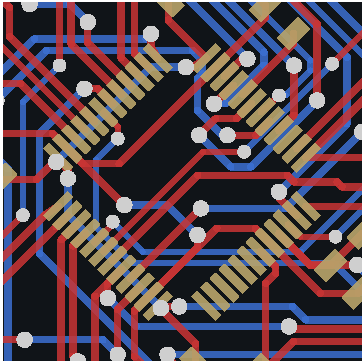
\includegraphics[width=\textwidth]{closeup.pdf}
    \caption{Close-up of fine-pitch QFN escapes on the motor-driver board (14\,mm square). Pads in gold.}
    \label{fig:closeup}
  \end{subfigure}\hfill
  \begin{subfigure}[t]{0.56\textwidth}
    \centering
    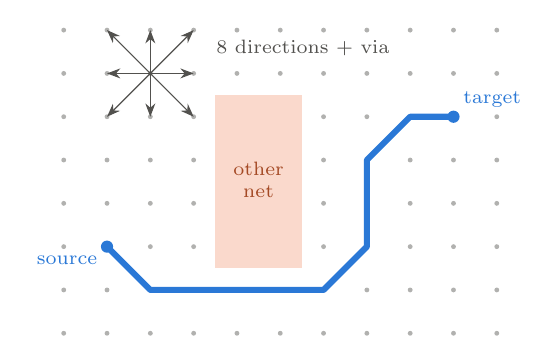
\begin{tikzpicture}[scale=0.55, every node/.style={font=\scriptsize}]
      \foreach \x in {0,...,10} \foreach \y in {0,...,7} \fill[ink2!45] (\x,\y) circle (1.6pt);
      \fill[frorange!25] (3.5,1.5) rectangle (5.5,5.5);
      \node[frorange!70!black] at (4.5,3.5) {\begin{tabular}{c}other\\net\end{tabular}};
      \fill[tmblue] (1,2) circle (4pt) node[below left] {source};
      \fill[tmblue] (9,5) circle (4pt) node[above right] {target};
      \draw[tmblue, line width=2.2pt, line cap=round, line join=round]
        (1,2) -- (2,1) -- (6,1) -- (7,2) -- (7,4) -- (8,5) -- (9,5);
      \draw[-{Stealth}, ink2] (2,6) -- (3,6); \draw[-{Stealth}, ink2] (2,6) -- (3,7);
      \draw[-{Stealth}, ink2] (2,6) -- (2,7); \draw[-{Stealth}, ink2] (2,6) -- (1,7);
      \draw[-{Stealth}, ink2] (2,6) -- (1,6); \draw[-{Stealth}, ink2] (2,6) -- (1,5);
      \draw[-{Stealth}, ink2] (2,6) -- (2,5); \draw[-{Stealth}, ink2] (2,6) -- (3,5);
      \node[ink2, align=left, anchor=west] at (3.3,6.6) {8 directions + via};
    \end{tikzpicture}
    \caption{Octilinear lattice search: each point has eight neighbours on its layer plus a via move; points within
    clearance of another net's copper (shaded) are not usable.}
    \label{fig:lattice}
  \end{subfigure}
  \caption{Detailed routing on the lattice.}
\end{figure}

\subsection{Learning from failure}
\label{sec:learning}

The requirement was to ``try the optimal first, store the failure information and use it to improve the next
attempt''. TraceMaker does this at four levels.

\begin{enumerate}[leftmargin=*]
  \item \textbf{Within a search.} A failed search reports \emph{why}: the source or target pad is boxed in (the
  open list ran out without reaching the window edge), the window was too small, the search budget ran out, or
  the exact check rejected the path. A boxed-in target is detected with a short reverse search from the target.
  The reason picks the next step instead of blindly retrying.
  \item \textbf{Escalation ladder per connection.} Strict routing first (no crossing of other copper); then forced
  off-lattice escapes for pads with no lattice exit; then a neck-down to the board's minimum track width; then
  negotiation.
  \item \textbf{Negotiated rip-up (PathFinder).} In negotiation a path may cross other connections' copper at a cost.
  The crossed connections are ripped up and queued again, and every contested lattice point accumulates a history
  cost
  \begin{equation}
    h_\text{hist}(v) \leftarrow h_\text{hist}(v) + 1 \quad\text{whenever } v \text{ is contested},
  \end{equation}
  so that later searches avoid congested places. This is the PathFinder idea of McMurchie and Ebeling (1995).
  ``Nogoods'' record attempts that failed in exactly the same surroundings, so they are not repeated, and the best
  legal state seen so far is always kept. When negotiation stalls, the router restarts from an empty board with
  the hardest connections first, keeping the history; once the planned restarts are used, further restarts clear
  the nogoods, halve the history and shuffle ties while budget remains.
  \item \textbf{Across runs.} A SQLite knowledge base stores, per class of board, how well each router variant did
  and which connections failed on each board. A Thompson-sampling bandit chooses variants: each variant $k$ has a
  Beta$(\alpha_k,\beta_k)$ posterior over its success rate, a sample $\theta_k$ is drawn for each, and the variants
  with the largest samples run. Connections that failed before are routed first next time.
\end{enumerate}

\begin{figure}[h]
\centering
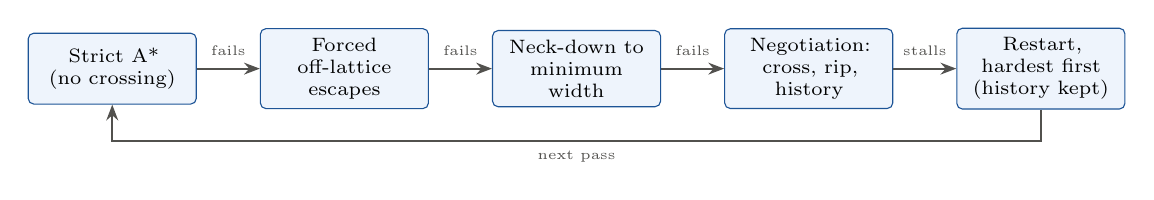
\begin{tikzpicture}[node distance=3mm and 8mm,
  st/.style={draw=tmblue!70!black, fill=boxfill, rounded corners=2pt, font=\scriptsize, align=center,
             minimum height=9mm, text width=19mm},
  arr/.style={-{Stealth[length=2mm]}, thick, ink2}]
  \node[st] (s1) {Strict A*\\(no crossing)};
  \node[st, right=of s1] (s2) {Forced\\off-lattice escapes};
  \node[st, right=of s2] (s3) {Neck-down to\\minimum width};
  \node[st, right=of s3] (s4) {Negotiation:\\cross, rip, history};
  \node[st, right=of s4] (s5) {Restart, hardest first\\(history kept)};
  \draw[arr] (s1) -- node[above=1pt, font=\tiny] {fails} (s2);
  \draw[arr] (s2) -- node[above=1pt, font=\tiny] {fails} (s3);
  \draw[arr] (s3) -- node[above=1pt, font=\tiny] {fails} (s4);
  \draw[arr] (s4) -- node[above=1pt, font=\tiny] {stalls} (s5);
  \draw[arr] (s5.south) -- ++(0,-4mm) -| node[pos=0.25, below, font=\tiny] {next pass} (s1.south);
\end{tikzpicture}
\caption{Escalation ladder for a connection that does not route. Each failure is classified, and the
classification decides the next rung.}
\label{fig:ladder}
\end{figure}

\subsection{Clean-up after routing}
\label{sec:cleanup}

Search on a lattice finds legal paths, but not tidy ones: equal-cost staircases of short 45\textdegree\ steps, and vias
placed where a slightly longer single-layer route existed. Once routing is done, TraceMaker therefore cleans up,
much as Freerouting's optimizer does:
\begin{enumerate}[leftmargin=*]
  \item \textbf{Via-saving re-routes.} Connections that use vias are taken out one at a time, most vias first, and
  routed again with vias made ten times dearer and other connections' copper as a hard obstacle. The new route is kept
  only if it is cheaper by track length plus 2\,mm per via; otherwise the old copper is restored exactly. Rounds
  repeat while connections improve and search budget remains.
  \item \textbf{Path smoothing (``pull tight'').} Within each connection, runs of same-layer, same-width segments are
  replaced by the fewest octilinear segments that the exact rule check accepts, keeping pads and vias where they
  are. This step is pure geometry, cheap and deterministic, so it always runs.
\end{enumerate}
Every new segment passes the same exact check as during routing, so clean-up cannot introduce a DRC error.

\subsection{Parallel portfolio and determinism}

Different strategies suit different boards: short connections first or long first, cheap or expensive vias,
exact bend tracking or fast bends, and on large boards a lattice of double pitch. TraceMaker runs a portfolio of
eight such variants in parallel threads and keeps the best result (most connections, then fewest vias, then
shortest copper). When one variant has routed everything after time $T$, the others may continue until $2T + 5$\,s, so
a cleaner complete result can still win.

Runs can be made fully deterministic with a work budget (\texttt{--work}, counted in A* expansions) instead of a
time limit: random choices use a counter-based Philox generator keyed by (seed, stage, item), hash containers are
never iterated in an output-affecting order, and costs are integers. Repeated runs then produce byte-identical
boards, which the regression tests rely on.

\subsection{GPU cost-to-go fields}
\label{sec:gpu}

On large search windows A* spends most of its time exploring around obstacles that a straight-line estimate does
not see. Before such a search, a CUDA kernel computes the exact obstacle-aware cost to the target from every
lattice point of the window (iterated GAMER-style sweeps over the grid). This field is a lower bound that is much
tighter than the octile distance, so A* expands far fewer points. The field never prunes: where it claims
``unreachable'', the router falls back to the octile bound, so the search stays complete. A CPU implementation
produces bit-identical fields, and the tests compare them. Because the GPUs are shared with other jobs, a variant
stops building fields if they take more than 30\% of its wall-clock time.

\subsection{Component placement}

Placement (\texttt{tracemaker-place}) works in stages: a quadratic wirelength minimisation with the bound-to-bound
net model, solved by conjugate gradients; SimPL-style spreading to remove overlap; rotation choice; legalisation to
the nearest legal position (courtyards, board outline, copper and solder-mask clearances); and parallel simulated
annealing on half-perimeter wirelength
\begin{equation}
  \mathrm{HPWL} = \sum_{\text{nets } e} \Big(\max_{p\in e} x_p - \min_{p\in e} x_p + \max_{p\in e} y_p - \min_{p\in e} y_p\Big)
\end{equation}
plus a penalty per airwire crossing. A linear-programming lower bound on HPWL, solved as a min-cost flow, is reported
alongside so the quality of each placement can be judged.

Shorter wiring does not automatically mean a board routes better: denser packing can block escape routes. The
placer therefore puts the router in the loop. With \texttt{--route-check}, the input placement and the new one are
routed with the same deterministic budget, and the new placement is kept only if it leaves no more connections
unrouted. \texttt{--mode auto} does this for both the refine and the full mode and keeps the best of the three.

\subsection{Live view and KiCad integration}

\texttt{tracemaker route --view} streams the routing as it happens to a WebGL2 viewer in the browser: tracks
appearing and being ripped up, the A* frontier, failures and the remaining airwires. A KiCad~10 action plugin
routes the open board through KiCad's IPC API and adds the result in one undoable commit.

% ------------------------------------------------------------------------------------------------------------
\section{How it was tested}
\label{sec:testing}

\begin{itemize}[leftmargin=*]
  \item \textbf{Unit and integration tests} (43, run with \texttt{ctest}): exact unit conversion, Philox known-answer
  vectors, GPU-equals-CPU for the random generator and cost-to-go fields, s-expression parsing and byte-exact
  round trips, the board reader against KiCad's own model, rule reading, geometry predicates, placement legality
  and lower bounds, and the viewer server.
  \item \textbf{DRC parity.} TraceMaker's own DRC is compared with \texttt{kicad-cli} on the KiCad demo boards; 11 of 16
  match exactly on the 15 routing-relevant violation types, and these 11 are a regression test. The router uses the
  same rule engine, so parity problems show up as router errors and were fixed at the source.
  \item \textbf{Benchmark harness.} \texttt{bench/run.py} samples boards from Freerouting's PCBench set by
  Freerouting's own difficulty tiers, routes each with a snapshot of the binary (120\,s, eight variants), and runs
  \texttt{kicad-cli pcb drc} on the result. A board is \emph{clean} when it is fully connected and KiCad reports no
  violation involving a track, via or arc that was not already present in the unrouted board. The result is
  compared with Freerouting's published per-board results for the same files.
\end{itemize}

% ------------------------------------------------------------------------------------------------------------
\section{Results}

\subsection{Clean pass by tier}

Figure~\ref{fig:tiers} and Table~\ref{tab:tiers} give the final run (\texttt{final9}, with the clean-up stage). TraceMaker matches
Freerouting 2.5.0-RC12 on the routine tier-A boards and is ahead on the harder tiers. No board has a
router-introduced DRC error.

\begin{figure}[h]
  \centering
  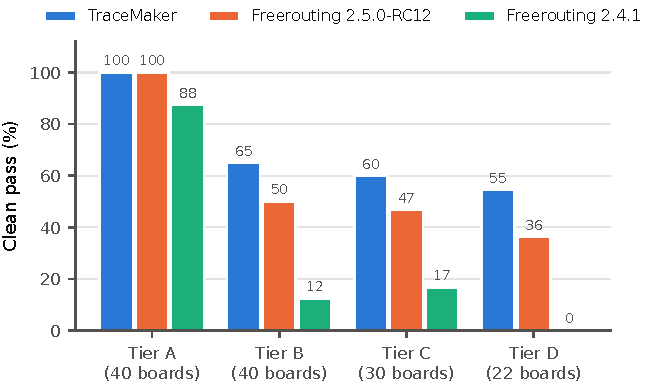
\includegraphics[width=0.75\textwidth]{tiers.pdf}
  \caption{Share of boards routed clean (fully connected, no router-introduced KiCad DRC errors), 120\,s per board.
  Freerouting figures are its published results on the same fixture files.}
  \label{fig:tiers}
\end{figure}

\begin{table}[h]
\centering
\small
\begin{tabular}{lrrrrr}
\toprule
Tier & Boards & TraceMaker & FR 2.5.0-RC12 & FR 2.4.1 & Router errors \\
\midrule
A (routine 2-layer)  & 40 & \textbf{100\%}  & 100\%  & 87.5\% & 0 \\
B (2--4 layer)       & 40 & \textbf{65.0\%} & 50.0\% & 12.5\% & 0 \\
C (complex)          & 30 & \textbf{60.0\%} & 46.7\% & 16.7\% & 0 \\
D (hardest)          & 22 & \textbf{54.5\%} & 36.4\% & 0.0\%  & 0 \\
\bottomrule
\end{tabular}
\caption{Final benchmark run. Samples: 40 of 453 tier-A boards, 40 of 560 tier-B, 30 of 122 tier-C and all 22
tier-D boards (fixed seed). FR: Freerouting's published results. Router errors: boards with router-introduced DRC errors.}
\label{tab:tiers}
\end{table}

Figure~\ref{fig:h2h} compares the two routers board by board. On every tier there are more boards that only
TraceMaker routes clean than boards that only Freerouting does.

\begin{figure}[h]
  \centering
  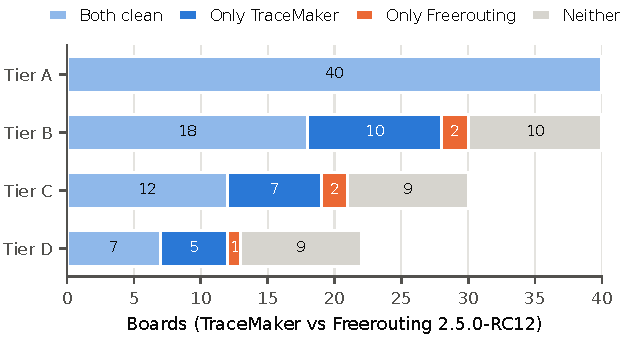
\includegraphics[width=0.75\textwidth]{head_to_head.pdf}
  \caption{Board-by-board comparison with Freerouting 2.5.0-RC12 in the final run.}
  \label{fig:h2h}
\end{figure}

\subsection{Progress during development}

Figure~\ref{fig:progress} tracks every full benchmark run during the development session. The first router
(plain lattice A*) routed 70\% of tier A clean. Fixing rule semantics found against KiCad, the learning mechanisms
and the escalation ladder took tier A to 100\% within about two and a half hours; the later gains on tiers B--D came from
boxed-in detection at both ends of a connection, pad-approach fixes for fine-pitch parts, the coarse-lattice
variants for large boards, extra restarts and the large-board setup fix.

\begin{figure}[h]
  \centering
  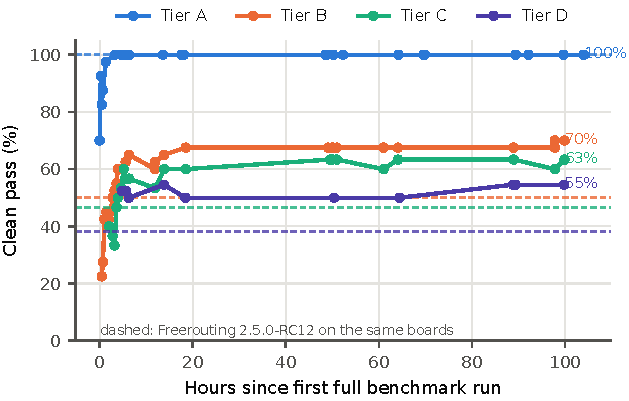
\includegraphics[width=0.75\textwidth]{progress.pdf}
  \caption{Clean pass of every full benchmark run (20 or more boards) over the development session. Dashed lines:
  Freerouting 2.5.0-RC12 on the same boards. Small run-to-run differences come from the wall-clock limit.}
  \label{fig:progress}
\end{figure}

\subsection{Completion and speed}

Clean pass is all-or-nothing. Figure~\ref{fig:completion} shows how close the remaining boards are: most boards
that are not clean miss only a few connections, and mean completion is above 95\% on every tier.

\begin{figure}[h]
  \centering
  \begin{subfigure}[t]{0.60\textwidth}
    \centering
    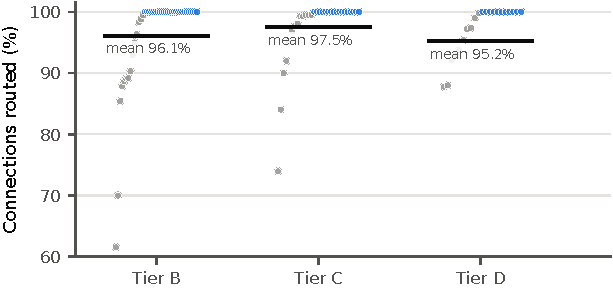
\includegraphics[width=\textwidth]{completion.pdf}
    \caption{Share of connections routed per board. Blue: fully routed.}
    \label{fig:completion}
  \end{subfigure}\hfill
  \begin{subfigure}[t]{0.38\textwidth}
    \centering
    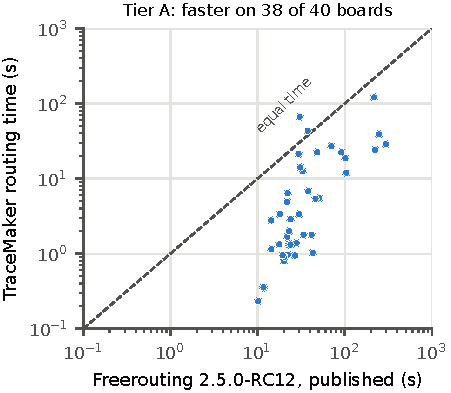
\includegraphics[width=\textwidth]{time.pdf}
    \caption{Tier-A routing time against Freerouting's published time.}
    \label{fig:time}
  \end{subfigure}
  \caption{Completion on the harder tiers and speed on tier A. Freerouting's times were measured on its own
  hardware, so the comparison is indicative only; TraceMaker used eight threads of a 56-core server.}
\end{figure}

On tier A the median TraceMaker routing time is 2.5\,s per board (5.9\,s including file input and output; the
clean-up stage and the grace period for other portfolio variants added about 2\,s), and
every board finished faster than Freerouting's published time (Figure~\ref{fig:time}).

\subsection{Routed boards}

Figure~\ref{fig:boards} shows a selection of routed boards from the final run, rendered from the output files.
The four-layer high-voltage switching board (604 connections) uses the inner layers (yellow and green);
\texttt{draco} and \texttt{EUC-VESC} are boards that TraceMaker routes clean and Freerouting does not.

\begin{figure}[htbp]
  \centering
  \begin{subfigure}[t]{0.48\textwidth}
    \centering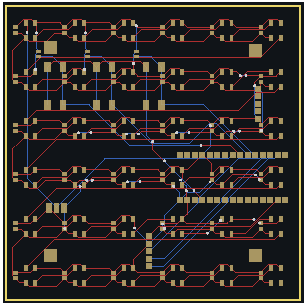
\includegraphics[width=\textwidth]{board_a.pdf}
    \caption{\texttt{Hangul-Clock} (tier A): 209 connections, 18\,s.}
  \end{subfigure}\hfill
  \begin{subfigure}[t]{0.48\textwidth}
    \centering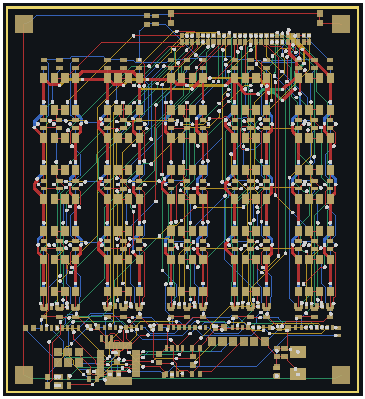
\includegraphics[width=\textwidth]{board_c.pdf}
    \caption{\texttt{40-channel-hv-switching-board} (tier C, 4 layers): 604 connections.}
  \end{subfigure}\\[4mm]
  \begin{subfigure}[t]{0.48\textwidth}
    \centering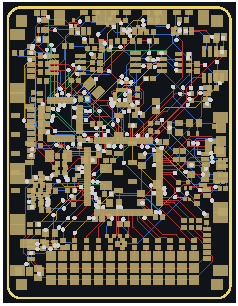
\includegraphics[width=\textwidth]{board_draco.pdf}
    \caption{\texttt{draco} (tier C): 418 connections; clean only with TraceMaker.}
  \end{subfigure}\hfill
  \begin{subfigure}[t]{0.48\textwidth}
    \centering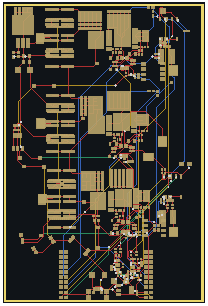
\includegraphics[width=\textwidth]{board_d.pdf}
    \caption{\texttt{EUC-VESC} (tier D): 760 connections; clean only with TraceMaker.}
  \end{subfigure}
  \caption{Boards routed by TraceMaker in the final benchmark run, each fully connected with no router-introduced
  KiCad DRC errors. Red: front copper; blue: back copper; yellow and green: inner layers; gold: pads; grey: vias.}
  \label{fig:boards}
\end{figure}

\subsection{Placement}

The placer was evaluated on 23 PCBench boards in \texttt{--mode auto} with a router check of three million A*
expansions (Figure~\ref{fig:placement}). It kept a new placement on 18 boards and the human placement on five.
Total HPWL fell from 17,464\,mm to 13,190\,mm ($-24.5\%$, median $-17\%$ per board), unrouted connections fell from
61 to 59, and no board got worse. Without the router check, placement alone cut wirelength by a similar amount
but left 13 boards fully routed instead of 15: denser packing can block routing, which is why the check exists.

\begin{figure}[h]
  \centering
  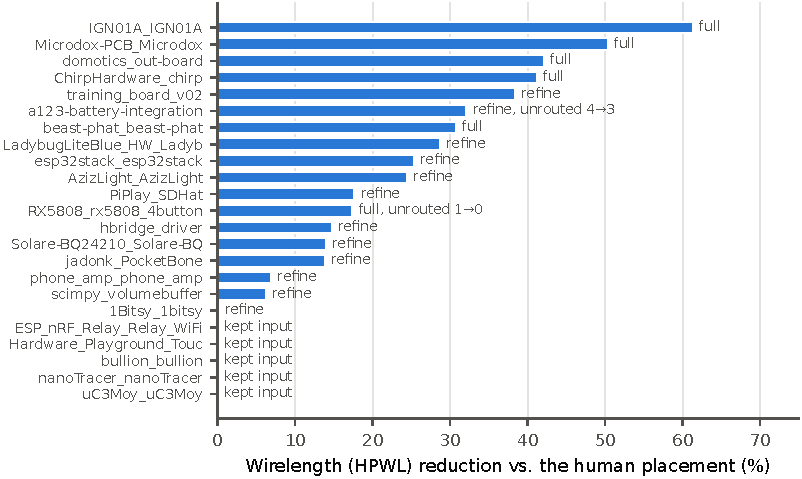
\includegraphics[width=0.9\textwidth]{placement.pdf}
  \caption{Wirelength reduction of the placement kept by \texttt{tracemaker-place --mode auto}, per board. ``Kept input'':
  the router check kept the human placement. Labels give the mode kept and any change in unrouted connections.}
  \label{fig:placement}
\end{figure}


\subsection{Quality benchmark on held-out boards}
\label{sec:quality}

The tier results above come from boards that were used while TraceMaker was developed, and compare against
Freerouting's published numbers. To remove both weaknesses, 60 PCBench boards that never appeared in any development
run (20 each from tiers A, B and C, fixed random seed) were routed by TraceMaker, Freerouting 2.5.0-RC12 and
Freerouting 1.9.0 on the same machine. Freerouting used its published settings (one thread, 500 passes, fanout and
optimizer on, 30-minute limit) on the fixture's Specctra file, and its result was imported into the KiCad board.
(``2.5.0-RC12'' is the name of the jar in Freerouting's own benchmark set; the program reports itself as
v2.4.2-SNAPSHOT, built 2026-09-29.)
Every result was judged by KiCad's DRC and measured by the same quality script (\texttt{bench/quality.py}); the
human-routed originals were measured as a reference.

\begin{table}[h]
\centering
\small
\begin{tabular}{lrrrrr}
\toprule
Router & KiCad clean & Connected & Completion & Router errors & Median time \\
\midrule
TraceMaker & \textbf{73\%} & 73\% & 98.3\% & \textbf{0} & 38\,s \\
Freerouting 2.5.0-RC12 & 3\% & 78\% & 97.4\% & 58 & 24\,s \\
Freerouting 1.9.0 & 32\% & 66\% & 96.8\% & 34 & 191\,s \\
Human original & 3\% & 77\% & 98.0\% & 58 & -- \\
\bottomrule
\end{tabular}
\caption{Held-out quality benchmark, 60 boards (\texttt{quality-3}). Three TraceMaker runs of the same boards
gave 72--78\% clean, so differences of a few points are within run-to-run variation. ``Router errors'': boards with
router-introduced KiCad DRC errors; TraceMaker includes the clean-up stage. Freerouting 1.9.0 failed to
produce a result on one board.}
\label{tab:quality}
\end{table}

\begin{figure}[h]
  \centering
  \begin{subfigure}[t]{0.52\textwidth}
    \centering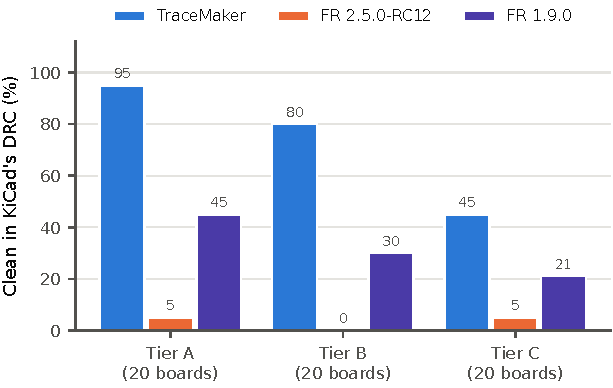
\includegraphics[width=\textwidth]{quality_clean.pdf}
    \caption{Clean in KiCad's DRC, by tier.}
  \end{subfigure}\hfill
  \begin{subfigure}[t]{0.46\textwidth}
    \centering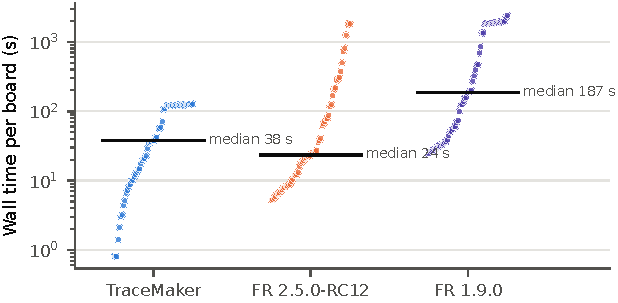
\includegraphics[width=\textwidth]{quality_time.pdf}
    \caption{Wall time per board (recorded, not optimised for).}
  \end{subfigure}
  \caption{Held-out boards: correctness and time.}
  \label{fig:qclean}
\end{figure}

\begin{figure}[h]
  \centering
  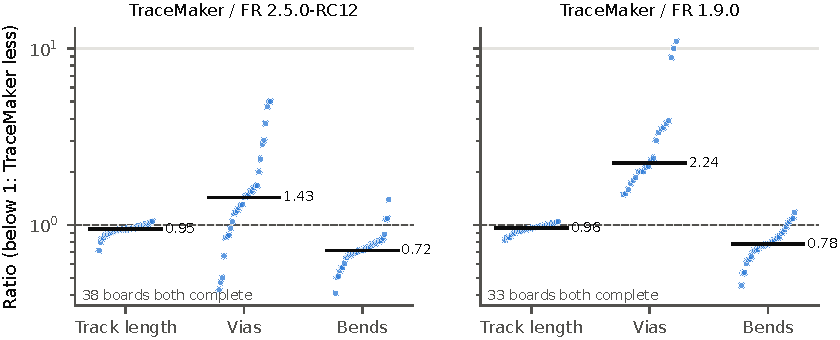
\includegraphics[width=\textwidth]{quality_ratios.pdf}
  \caption{Layout quality on boards that both routers fully connected: TraceMaker's value divided by Freerouting's,
  one dot per board; the bar is the median.}
  \label{fig:qratios}
\end{figure}

\noindent What the held-out benchmark shows:
\begin{itemize}[leftmargin=*]
  \item \textbf{Correctness is TraceMaker's clearest advantage.} No TraceMaker result had a router-introduced KiCad
  error. Freerouting connects about as many boards, but almost none of its results pass KiCad's DRC. On 38 of the 60
  boards Freerouting 2.5's only errors are board-edge clearance or tracks below the minimum width, rules that KiCad's
  Specctra export does not pass on; both Freerouting versions also had genuine clearance errors on 9--10 boards and
  shorts on 3--4.
  \item \textbf{Connection rate is about equal.} TraceMaker fully connected 73--78\% of boards across runs,
  Freerouting 2.5 78\% and Freerouting 1.9 66\%.
  \item \textbf{Layout quality is mixed.} Against Freerouting 2.5, TraceMaker's tracks are 5\% shorter and it has 28\%
  fewer bends, but 43\% more vias (medians over 38 boards both completed). Against Freerouting 1.9 its tracks are 4\%
  shorter with 22\% fewer bends, but 2.2 times the vias. The clean-up stage cut the via ratio from 2.15 to 1.43 and the
  bend ratio from 1.20 to 0.72 against Freerouting 2.5.
  \item \textbf{Acute angles:} TraceMaker had none outside pad copper on any board; Freerouting 2.5 had 9 and
  Freerouting 1.9 had 7 in total.
  \item \textbf{The held-out set found two real bugs.} Text drawn on a solder-mask layer opens the mask; routing under
  it caused bridges on two boards before the fix.
\end{itemize}

\subsection{Head to head on one board}
\label{sec:h2h-board}

To compare layout quality and not only pass or fail, the tier-C board \texttt{AmpOne} (a two-layer audio amplifier,
321 connections) was routed by TraceMaker, Freerouting 2.5.0-RC12 and Freerouting 1.9.0 on the same machine, and measured together
with the human-routed original (Figures~\ref{fig:cmp} and~\ref{fig:cmpzoom}, Table~\ref{tab:cmp}). Freerouting ran
with its published benchmark settings (one thread, up to 500 passes, fanout and optimizer on, 30-minute limit) from
the fixture's Specctra file, and its session was imported back into the KiCad board, so KiCad's DRC and the same
quality metrics judge every result.

\begin{figure}[h]
  \centering
  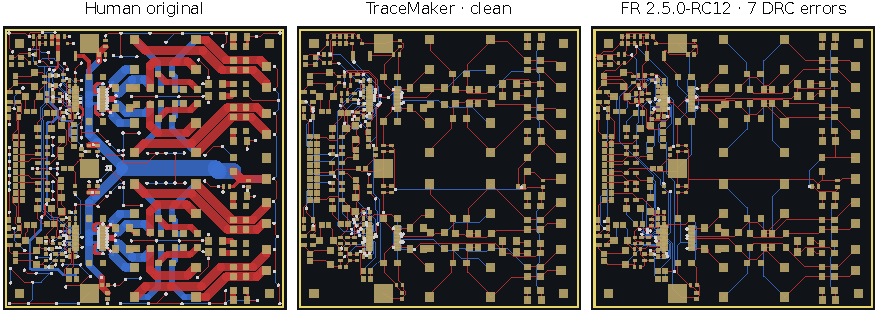
\includegraphics[width=0.92\textwidth]{compare_AmpOne_dev-AmpOne.pdf}
  \caption{\texttt{AmpOne} routed four ways. The human design uses very wide power tracks; none of the routers does,
  because the board's net classes do not ask for them.}
  \label{fig:cmp}
\end{figure}

\begin{figure}[h]
  \centering
  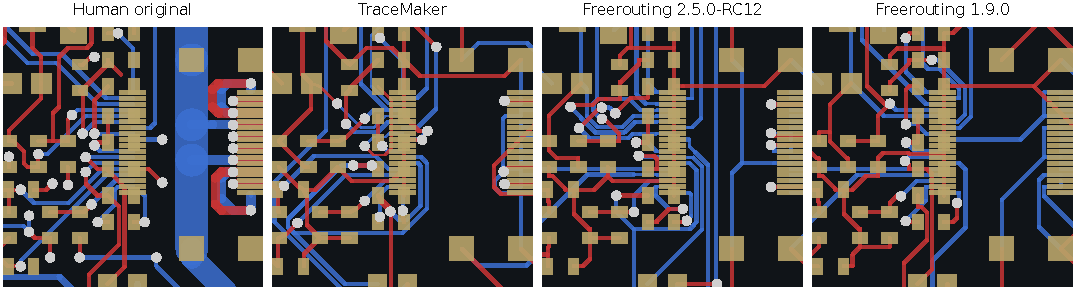
\includegraphics[width=\textwidth]{compare_AmpOne_dev-AmpOne_zoom.pdf}
  \caption{The same 22\,mm window, centred on the densest pad area, in each result.}
  \label{fig:cmpzoom}
\end{figure}

\begin{table}[h]
\centering
\small
\begin{tabular}{lrrr}
\toprule
 & Human original & TraceMaker & FR 2.5.0-RC12 \\
\midrule
Connections routed & 100.0\% & 100.0\% & 100.0\% \\
Router-introduced DRC errors & n/a & 0 & 7 \\
Track length (mm) & 3,179 & 2,564 & 2,714 \\
Length / pad MST & 1.43 & 1.15 & 1.22 \\
Vias & 258 & 90 & 42 \\
Bends & 669 & 1,103 & 723 \\
Turns sharper than 90\textdegree & 17 & 33 & 0 \\
Narrowed track (mm) & 2.0 & 64.9 & 40.2 \\
Wall time (s) & -- & 46 & 37 \\
\bottomrule
\end{tabular}

\caption{Quality metrics for \texttt{AmpOne}. ``Length / pad MST'' divides the track length by the length of a
minimum spanning tree over each net's pad centres. ``Narrowed'' is track thinner than the net's design width. Acute angles count joints of two tracks of the same
net at less than 90\textdegree; only those outside pad copper are etchant traps.
The human original is shown for reference: it does not pass the board's own rules (371 clearance errors).}
\label{tab:cmp}
\end{table}

\noindent A video of all three routers working on this board, played at 4$\times$ real time, is in
\texttt{report/compare\_AmpOne.mp4}.

\noindent What the comparison shows:
\begin{itemize}[leftmargin=*]
  \item \textbf{All three routers connect everything; only TraceMaker passes KiCad's DRC.} Freerouting 2.5.0-RC12 leaves
  three hole-clearance and four board-edge-clearance errors, and Freerouting 1.9.0 seven board-edge-clearance errors.
  Both report their own result clean: the Specctra file they route from does not carry all of KiCad's rules.
  \item \textbf{TraceMaker uses the least copper and the fewest bends.} Its tracks are 4\% shorter than Freerouting
  2.5's, 6\% shorter than Freerouting 1.9's and 18\% shorter than the human routing, with 594 bends against 723 and 610.
  \item \textbf{Freerouting uses fewer vias.} TraceMaker uses 59 vias, Freerouting 2.5 42 and Freerouting 1.9 23. Before
  the clean-up stage (Section~\ref{sec:cleanup}) TraceMaker used 90 vias and about 1,100 bends on this board.
  TraceMaker joins 20 track pairs at acute angles at pad centres, where the pad's copper fills the angle, and has none
  outside a pad (Freerouting 1.9 has one, the human routing nine). It narrows 97\,mm of track below the design width
  to pass tight spots.
  \item \textbf{Speed:} TraceMaker 78\,s with eight threads, Freerouting 2.5 39\,s and Freerouting 1.9 394\,s, each
  with one thread.
\end{itemize}

% ------------------------------------------------------------------------------------------------------------
\section{Limitations and next steps}
\label{sec:limits}

\begin{itemize}[leftmargin=*]
  \item \textbf{Large boards are time-limited.} On the biggest boards the router finishes only one or two negotiation
  passes in 120\,s; an A* expansion costs about 430\,ns. Global routing corridors, a coarse-to-fine lattice and
  parallelism inside one route are the next steps.
  \item \textbf{Edge-connector fingers under solder-mask openings} are left unrouted rather than routed with
  mask bridges. On the PCIe adapter board KiCad flags any track leaving the fingers, and the human-routed original
  has 16 such bridges itself. Freerouting's published ``clean'' counts only clearance violations and unrouted
  connections, so on these boards TraceMaker is judged more strictly.
  \item \textbf{More vias than Freerouting.} Even after clean-up TraceMaker uses about 1.4 times Freerouting 2.5's vias
  and 2.2 times Freerouting 1.9's (median, held-out boards), and it narrows some tracks below the design width.
  Layer-direction preferences and a via-minimising global stage are the next levers.
  \item \textbf{The tier statistics use Freerouting's published numbers,} which allowed up to 30 minutes per board and
  are judged by Freerouting's own DRC. The held-out quality benchmark (Section~\ref{sec:quality}) runs both
  Freerouting versions locally and judges them with KiCad, but covers 60 boards; tier D has no unused boards left.
  \item \textbf{Copper text} is modelled by generous estimated boxes rather than exact glyph outlines.
  \item \textbf{Placement} does not yet have a routability term inside the annealer, side flipping or
  decoupling-capacitor grouping.
  \item \textbf{Not yet built:} schematic-to-board flow, escape planning for large BGAs, differential-pair and
  length tuning.
\end{itemize}

% ------------------------------------------------------------------------------------------------------------
\appendix
\section{Reproducing the results}
\begin{small}
\begin{verbatim}
cmake --preset release && cmake --build --preset release && ctest --preset release
scripts/fetch_fixtures.sh pcbench
python3 bench/run.py --tier B --limit 40 --time 120 --jobs 2 --threads 8 --name my-run
build/release/src/app/tracemaker route board.kicad_pcb -o routed.kicad_pcb --time 120 --view
build/release/src/place/tracemaker-place in.kicad_pcb -o out.kicad_pcb \
    --mode auto --route-check 3000000
build/report-venv/bin/python report/make_figures.py   # figures for this report
\end{verbatim}
\end{small}

\end{document}
